\chapter{Seção de Primeiro Nível}\label{section:1}

	Lorem ipsum dolor sit amet, consectetur adipiscing elit. Nullam quis ante varius, scelerisque eros id, tincidunt sem. Nam tincidunt porttitor mauris id aliquam. Aenean facilisis, diam vitae luctus tincidunt, lacus nisi dapibus leo, a feugiat tortor ipsum a mauris. Curabitur id velit condimentum, lacinia arcu in, ultrices augue. Aenean vitae velit efficitur tellus venenatis maximus. Nam facilisis ornare ipsum at dapibus. Fusce ut ligula sed dui dapibus porta. Vivamus viverra tortor hendrerit ante facilisis sodales. Ut et dignissim orci, ac tempor felis. Cras ex felis, facilisis ut gravida interdum, consectetur a ligula.

	Etiam dignissim lorem eget libero dictum convallis. Nulla sit amet varius neque, in pulvinar eros. Nam dignissim tristique consectetur. Suspendisse aliquam rhoncus lacus sed dictum. Donec malesuada, nisi nec tempor fermentum, nisi tellus venenatis ante, non porta sapien erat et felis. Fusce suscipit malesuada mi, rutrum rhoncus purus hendrerit nec. Mauris tempor luctus tempus. Suspendisse consectetur vehicula turpis. Morbi sed ipsum nec arcu hendrerit auctor vel id magna. Sed ac ex dolor. Sed quis urna ipsum. Curabitur sit amet venenatis purus. Quisque commodo risus at justo mattis, in eleifend libero fermentum. Maecenas velit erat, pellentesque ut aliquam vel, facilisis sed arcu. Phasellus feugiat tortor purus, sed viverra magna venenatis eu. Mauris ultrices mauris et diam interdum, id consectetur ligula blandit.

	Curabitur consequat, ipsum iaculis tincidunt consequat, est leo condimentum felis, et pretium purus turpis quis tellus. In mollis, elit nec vestibulum cursus, nisl magna scelerisque lorem, sed egestas odio justo sed lectus. Etiam vel lorem sit amet elit ultricies rhoncus. Phasellus eu eleifend ligula. Etiam sagittis dolor sit amet magna ultrices, non mollis nibh lobortis. Donec nec est aliquet, pulvinar nibh quis, varius arcu. Mauris finibus, odio eget hendrerit semper, dolor eros placerat lectus, ac blandit arcu ex sit amet nibh. Donec eu ante mi. Nulla mollis mollis congue. Fusce ac elit vel nisi gravida fringilla. In non mattis risus, pharetra luctus est. Aliquam erat volutpat. Sed in mi odio. Cras sit amet lacus eget elit sodales pulvinar at quis nibh.

	Cras nec nulla purus. Integer lectus odio, posuere at suscipit vel, vehicula vel justo. Aliquam magna tortor, consequat id ligula nec, condimentum sagittis leo. Proin eleifend sapien vel nulla vehicula euismod. In sed tempor ante, eu malesuada felis. Nunc non vulputate est, eu tincidunt sem. Nullam et nisl diam. Mauris semper, ex quis finibus eleifend, nisi turpis eleifend turpis, eu placerat ligula massa tempor lectus. Donec facilisis pretium enim a tempus. Sed ac erat nibh. Curabitur vitae felis mollis ex facilisis volutpat eu a purus. Nam in pulvinar erat.

	Curabitur feugiat justo at porttitor placerat. Nulla eget efficitur mi, non iaculis augue. Nunc eleifend ante sed mauris semper lobortis. In mauris mauris, dignissim et elit et, interdum rhoncus ante. Praesent commodo sem tortor, sodales pellentesque mi ultricies eget. Donec interdum augue in ex cursus, ultricies euismod est molestie. Integer diam lectus, consectetur a lacinia vel, eleifend eu magna. In hac habitasse platea dictumst. In ex magna, sodales ornare quam ut, tristique malesuada risus. Suspendisse scelerisque velit ut turpis condimentum, eget euismod risus tristique. Duis viverra tortor at egestas aliquam. Nam ut lobortis libero. Donec ut velit pretium, condimentum felis et, auctor leo. Maecenas a tellus justo. Integer eleifend, ante vel consectetur feugiat, odio felis ultricies dolor, et tristique turpis libero auctor elit. Phasellus et lacus lectus. 
	
	\section{\esp Seção de Segundo Nível}\label{section:1.1}
	
		Lorem ipsum dolor sit amet, consectetur adipiscing elit. Nullam quis ante varius, scelerisque eros id, tincidunt sem. Nam tincidunt porttitor mauris id aliquam. Aenean facilisis, diam vitae luctus tincidunt, lacus nisi dapibus leo, a feugiat tortor ipsum a mauris. Curabitur id velit condimentum, lacinia arcu in, ultrices augue. Aenean vitae velit efficitur tellus venenatis maximus. Nam facilisis ornare ipsum at dapibus. Fusce ut ligula sed dui dapibus porta. Vivamus viverra tortor hendrerit ante facilisis sodales. Ut et dignissim orci, ac tempor felis. Cras ex felis, facilisis ut gravida interdum, consectetur a ligula.

		Etiam dignissim lorem eget libero dictum convallis. Nulla sit amet varius neque, in pulvinar eros. Nam dignissim tristique consectetur. Suspendisse aliquam rhoncus lacus sed dictum. Donec malesuada, nisi nec tempor fermentum, nisi tellus venenatis ante, non porta sapien erat et felis. Fusce suscipit malesuada mi, rutrum rhoncus purus hendrerit nec. Mauris tempor luctus tempus. Suspendisse consectetur vehicula turpis. Morbi sed ipsum nec arcu hendrerit auctor vel id magna. Sed ac ex dolor. Sed quis urna ipsum. Curabitur sit amet venenatis purus. Quisque commodo risus at justo mattis, in eleifend libero fermentum. Maecenas velit erat, pellentesque ut aliquam vel, facilisis sed arcu. Phasellus feugiat tortor purus, sed viverra magna venenatis eu. Mauris ultrices mauris et diam interdum, id consectetur ligula blandit.

		Curabitur consequat, ipsum iaculis tincidunt consequat, est leo condimentum felis, et pretium purus turpis quis tellus. In mollis, elit nec vestibulum cursus, nisl magna scelerisque lorem, sed egestas odio justo sed lectus. Etiam vel lorem sit amet elit ultricies rhoncus. Phasellus eu eleifend ligula. Etiam sagittis dolor sit amet magna ultrices, non mollis nibh lobortis. Donec nec est aliquet, pulvinar nibh quis, varius arcu. Mauris finibus, odio eget hendrerit semper, dolor eros placerat lectus, ac blandit arcu ex sit amet nibh. Donec eu ante mi. Nulla mollis mollis congue. Fusce ac elit vel nisi gravida fringilla. In non mattis risus, pharetra luctus est. Aliquam erat volutpat. Sed in mi odio. Cras sit amet lacus eget elit sodales pulvinar at quis nibh.

		Cras nec nulla purus. Integer lectus odio, posuere at suscipit vel, vehicula vel justo. Aliquam magna tortor, consequat id ligula nec, condimentum sagittis leo. Proin eleifend sapien vel nulla vehicula euismod. In sed tempor ante, eu malesuada felis. Nunc non vulputate est, eu tincidunt sem. Nullam et nisl diam. Mauris semper, ex quis finibus eleifend, nisi turpis eleifend turpis, eu placerat ligula massa tempor lectus. Donec facilisis pretium enim a tempus. Sed ac erat nibh. Curabitur vitae felis mollis ex facilisis volutpat eu a purus. Nam in pulvinar erat.

		Curabitur feugiat justo at porttitor placerat. Nulla eget efficitur mi, non iaculis augue. Nunc eleifend ante sed mauris semper lobortis. In mauris mauris, dignissim et elit et, interdum rhoncus ante. Praesent commodo sem tortor, sodales pellentesque mi ultricies eget. Donec interdum augue in ex cursus, ultricies euismod est molestie. Integer diam lectus, consectetur a lacinia vel, eleifend eu magna. In hac habitasse platea dictumst. In ex magna, sodales ornare quam ut, tristique malesuada risus. Suspendisse scelerisque velit ut turpis condimentum, eget euismod risus tristique. Duis viverra tortor at egestas aliquam. Nam ut lobortis libero. Donec ut velit pretium, condimentum felis et, auctor leo. Maecenas a tellus justo. Integer eleifend, ante vel consectetur feugiat, odio felis ultricies dolor, et tristique turpis libero auctor elit. Phasellus et lacus lectus.
		
		\subsection{\esp Seção de Terceiro Nível}\label{section:1.1.1}
		
			Lorem ipsum dolor sit amet, consectetur adipiscing elit. Nullam quis ante varius, scelerisque eros id, tincidunt sem. Nam tincidunt porttitor mauris id aliquam. Aenean facilisis, diam vitae luctus tincidunt, lacus nisi dapibus leo, a feugiat tortor ipsum a mauris. Curabitur id velit condimentum, lacinia arcu in, ultrices augue. Aenean vitae velit efficitur tellus venenatis maximus. Nam facilisis ornare ipsum at dapibus. Fusce ut ligula sed dui dapibus porta. Vivamus viverra tortor hendrerit ante facilisis sodales. Ut et dignissim orci, ac tempor felis. Cras ex felis, facilisis ut gravida interdum, consectetur a ligula.

			Etiam dignissim lorem eget libero dictum convallis. Nulla sit amet varius neque, in pulvinar eros. Nam dignissim tristique consectetur. Suspendisse aliquam rhoncus lacus sed dictum. Donec malesuada, nisi nec tempor fermentum, nisi tellus venenatis ante, non porta sapien erat et felis. Fusce suscipit malesuada mi, rutrum rhoncus purus hendrerit nec. Mauris tempor luctus tempus. Suspendisse consectetur vehicula turpis. Morbi sed ipsum nec arcu hendrerit auctor vel id magna. Sed ac ex dolor. Sed quis urna ipsum. Curabitur sit amet venenatis purus. Quisque commodo risus at justo mattis, in eleifend libero fermentum. Maecenas velit erat, pellentesque ut aliquam vel, facilisis sed arcu. Phasellus feugiat tortor purus, sed viverra magna venenatis eu. Mauris ultrices mauris et diam interdum, id consectetur ligula blandit.

			Curabitur consequat, ipsum iaculis tincidunt consequat, est leo condimentum felis, et pretium purus turpis quis tellus. In mollis, elit nec vestibulum cursus, nisl magna scelerisque lorem, sed egestas odio justo sed lectus. Etiam vel lorem sit amet elit ultricies rhoncus. Phasellus eu eleifend ligula. Etiam sagittis dolor sit amet magna ultrices, non mollis nibh lobortis. Donec nec est aliquet, pulvinar nibh quis, varius arcu. Mauris finibus, odio eget hendrerit semper, dolor eros placerat lectus, ac blandit arcu ex sit amet nibh. Donec eu ante mi. Nulla mollis mollis congue. Fusce ac elit vel nisi gravida fringilla. In non mattis risus, pharetra luctus est. Aliquam erat volutpat. Sed in mi odio. Cras sit amet lacus eget elit sodales pulvinar at quis nibh.

			Cras nec nulla purus. Integer lectus odio, posuere at suscipit vel, vehicula vel justo. Aliquam magna tortor, consequat id ligula nec, condimentum sagittis leo. Proin eleifend sapien vel nulla vehicula euismod. In sed tempor ante, eu malesuada felis. Nunc non vulputate est, eu tincidunt sem. Nullam et nisl diam. Mauris semper, ex quis finibus eleifend, nisi turpis eleifend turpis, eu placerat ligula massa tempor lectus. Donec facilisis pretium enim a tempus. Sed ac erat nibh. Curabitur vitae felis mollis ex facilisis volutpat eu a purus. Nam in pulvinar erat.

			Curabitur feugiat justo at porttitor placerat. Nulla eget efficitur mi, non iaculis augue. Nunc eleifend ante sed mauris semper lobortis. In mauris mauris, dignissim et elit et, interdum rhoncus ante. Praesent commodo sem tortor, sodales pellentesque mi ultricies eget. Donec interdum augue in ex cursus, ultricies euismod est molestie. Integer diam lectus, consectetur a lacinia vel, eleifend eu magna. In hac habitasse platea dictumst. In ex magna, sodales ornare quam ut, tristique malesuada risus. Suspendisse scelerisque velit ut turpis condimentum, eget euismod risus tristique. Duis viverra tortor at egestas aliquam. Nam ut lobortis libero. Donec ut velit pretium, condimentum felis et, auctor leo. Maecenas a tellus justo. Integer eleifend, ante vel consectetur feugiat, odio felis ultricies dolor, et tristique turpis libero auctor elit. Phasellus et lacus lectus.
			
			\subsubsection{\esp  Seção de Quarto Nível}\label{section:1.1.1.1}
			
				Lorem ipsum dolor sit amet, consectetur adipiscing elit. Nullam quis ante varius, scelerisque eros id, tincidunt sem. Nam tincidunt porttitor mauris id aliquam. Aenean facilisis, diam vitae luctus tincidunt, lacus nisi dapibus leo, a feugiat tortor ipsum a mauris. Curabitur id velit condimentum, lacinia arcu in, ultrices augue. Aenean vitae velit efficitur tellus venenatis maximus. Nam facilisis ornare ipsum at dapibus. Fusce ut ligula sed dui dapibus porta. Vivamus viverra tortor hendrerit ante facilisis sodales. Ut et dignissim orci, ac tempor felis. Cras ex felis, facilisis ut gravida interdum, consectetur a ligula.

				Etiam dignissim lorem eget libero dictum convallis. Nulla sit amet varius neque, in pulvinar eros. Nam dignissim tristique consectetur. Suspendisse aliquam rhoncus lacus sed dictum. Donec malesuada, nisi nec tempor fermentum, nisi tellus venenatis ante, non porta sapien erat et felis. Fusce suscipit malesuada mi, rutrum rhoncus purus hendrerit nec. Mauris tempor luctus tempus. Suspendisse consectetur vehicula turpis. Morbi sed ipsum nec arcu hendrerit auctor vel id magna. Sed ac ex dolor. Sed quis urna ipsum. Curabitur sit amet venenatis purus. Quisque commodo risus at justo mattis, in eleifend libero fermentum. Maecenas velit erat, pellentesque ut aliquam vel, facilisis sed arcu. Phasellus feugiat tortor purus, sed viverra magna venenatis eu. Mauris ultrices mauris et diam interdum, id consectetur ligula blandit.

				Curabitur consequat, ipsum iaculis tincidunt consequat, est leo condimentum felis, et pretium purus turpis quis tellus. In mollis, elit nec vestibulum cursus, nisl magna scelerisque lorem, sed egestas odio justo sed lectus. Etiam vel lorem sit amet elit ultricies rhoncus. Phasellus eu eleifend ligula. Etiam sagittis dolor sit amet magna ultrices, non mollis nibh lobortis. Donec nec est aliquet, pulvinar nibh quis, varius arcu. Mauris finibus, odio eget hendrerit semper, dolor eros placerat lectus, ac blandit arcu ex sit amet nibh. Donec eu ante mi. Nulla mollis mollis congue. Fusce ac elit vel nisi gravida fringilla. In non mattis risus, pharetra luctus est. Aliquam erat volutpat. Sed in mi odio. Cras sit amet lacus eget elit sodales pulvinar at quis nibh.

				Cras nec nulla purus. Integer lectus odio, posuere at suscipit vel, vehicula vel justo. Aliquam magna tortor, consequat id ligula nec, condimentum sagittis leo. Proin eleifend sapien vel nulla vehicula euismod. In sed tempor ante, eu malesuada felis. Nunc non vulputate est, eu tincidunt sem. Nullam et nisl diam. Mauris semper, ex quis finibus eleifend, nisi turpis eleifend turpis, eu placerat ligula massa tempor lectus. Donec facilisis pretium enim a tempus. Sed ac erat nibh. Curabitur vitae felis mollis ex facilisis volutpat eu a purus. Nam in pulvinar erat.

				Curabitur feugiat justo at porttitor placerat. Nulla eget efficitur mi, non iaculis augue. Nunc eleifend ante sed mauris semper lobortis. In mauris mauris, dignissim et elit et, interdum rhoncus ante. Praesent commodo sem tortor, sodales pellentesque mi ultricies eget. Donec interdum augue in ex cursus, ultricies euismod est molestie. Integer diam lectus, consectetur a lacinia vel, eleifend eu magna. In hac habitasse platea dictumst. In ex magna, sodales ornare quam ut, tristique malesuada risus. Suspendisse scelerisque velit ut turpis condimentum, eget euismod risus tristique. Duis viverra tortor at egestas aliquam. Nam ut lobortis libero. Donec ut velit pretium, condimentum felis et, auctor leo. Maecenas a tellus justo. Integer eleifend, ante vel consectetur feugiat, odio felis ultricies dolor, et tristique turpis libero auctor elit. Phasellus et lacus lectus. 
				
				\paragraph{\esp Seção de Quinto Nível}\label{section:1.1.1.1.1}
				
					Lorem ipsum dolor sit amet, consectetur adipiscing elit. Nullam quis ante varius, scelerisque eros id, tincidunt sem. Nam tincidunt porttitor mauris id aliquam. Aenean facilisis, diam vitae luctus tincidunt, lacus nisi dapibus leo, a feugiat tortor ipsum a mauris. Curabitur id velit condimentum, lacinia arcu in, ultrices augue. Aenean vitae velit efficitur tellus venenatis maximus. Nam facilisis ornare ipsum at dapibus. Fusce ut ligula sed dui dapibus porta. Vivamus viverra tortor hendrerit ante facilisis sodales. Ut et dignissim orci, ac tempor felis. Cras ex felis, facilisis ut gravida interdum, consectetur a ligula.

					Etiam dignissim lorem eget libero dictum convallis. Nulla sit amet varius neque, in pulvinar eros. Nam dignissim tristique consectetur. Suspendisse aliquam rhoncus lacus sed dictum. Donec malesuada, nisi nec tempor fermentum, nisi tellus venenatis ante, non porta sapien erat et felis. Fusce suscipit malesuada mi, rutrum rhoncus purus hendrerit nec. Mauris tempor luctus tempus. Suspendisse consectetur vehicula turpis. Morbi sed ipsum nec arcu hendrerit auctor vel id magna. Sed ac ex dolor. Sed quis urna ipsum. Curabitur sit amet venenatis purus. Quisque commodo risus at justo mattis, in eleifend libero fermentum. Maecenas velit erat, pellentesque ut aliquam vel, facilisis sed arcu. Phasellus feugiat tortor purus, sed viverra magna venenatis eu. Mauris ultrices mauris et diam interdum, id consectetur ligula blandit.

					Curabitur consequat, ipsum iaculis tincidunt consequat, est leo condimentum felis, et pretium purus turpis quis tellus. In mollis, elit nec vestibulum cursus, nisl magna scelerisque lorem, sed egestas odio justo sed lectus. Etiam vel lorem sit amet elit ultricies rhoncus. Phasellus eu eleifend ligula. Etiam sagittis dolor sit amet magna ultrices, non mollis nibh lobortis. Donec nec est aliquet, pulvinar nibh quis, varius arcu. Mauris finibus, odio eget hendrerit semper, dolor eros placerat lectus, ac blandit arcu ex sit amet nibh. Donec eu ante mi. Nulla mollis mollis congue. Fusce ac elit vel nisi gravida fringilla. In non mattis risus, pharetra luctus est. Aliquam erat volutpat. Sed in mi odio. Cras sit amet lacus eget elit sodales pulvinar at quis nibh.

					Cras nec nulla purus. Integer lectus odio, posuere at suscipit vel, vehicula vel justo. Aliquam magna tortor, consequat id ligula nec, condimentum sagittis leo. Proin eleifend sapien vel nulla vehicula euismod. In sed tempor ante, eu malesuada felis. Nunc non vulputate est, eu tincidunt sem. Nullam et nisl diam. Mauris semper, ex quis finibus eleifend, nisi turpis eleifend turpis, eu placerat ligula massa tempor lectus. Donec facilisis pretium enim a tempus. Sed ac erat nibh. Curabitur vitae felis mollis ex facilisis volutpat eu a purus. Nam in pulvinar erat.

					Curabitur feugiat justo at porttitor placerat. Nulla eget efficitur mi, non iaculis augue. Nunc eleifend ante sed mauris semper lobortis. In mauris mauris, dignissim et elit et, interdum rhoncus ante. Praesent commodo sem tortor, sodales pellentesque mi ultricies eget. Donec interdum augue in ex cursus, ultricies euismod est molestie. Integer diam lectus, consectetur a lacinia vel, eleifend eu magna. In hac habitasse platea dictumst. In ex magna, sodales ornare quam ut, tristique malesuada risus. Suspendisse scelerisque velit ut turpis condimentum, eget euismod risus tristique. Duis viverra tortor at egestas aliquam. Nam ut lobortis libero. Donec ut velit pretium, condimentum felis et, auctor leo. Maecenas a tellus justo. Integer eleifend, ante vel consectetur feugiat, odio felis ultricies dolor, et tristique turpis libero auctor elit. Phasellus et lacus lectus. 


\chapter{Instruções}\label{section:2}
	
	\section{\esp Declaração de Fotos}\label{section:2.1}

		\begin{center}
			\centering	
			\fotos{Exemplo de Foto}
			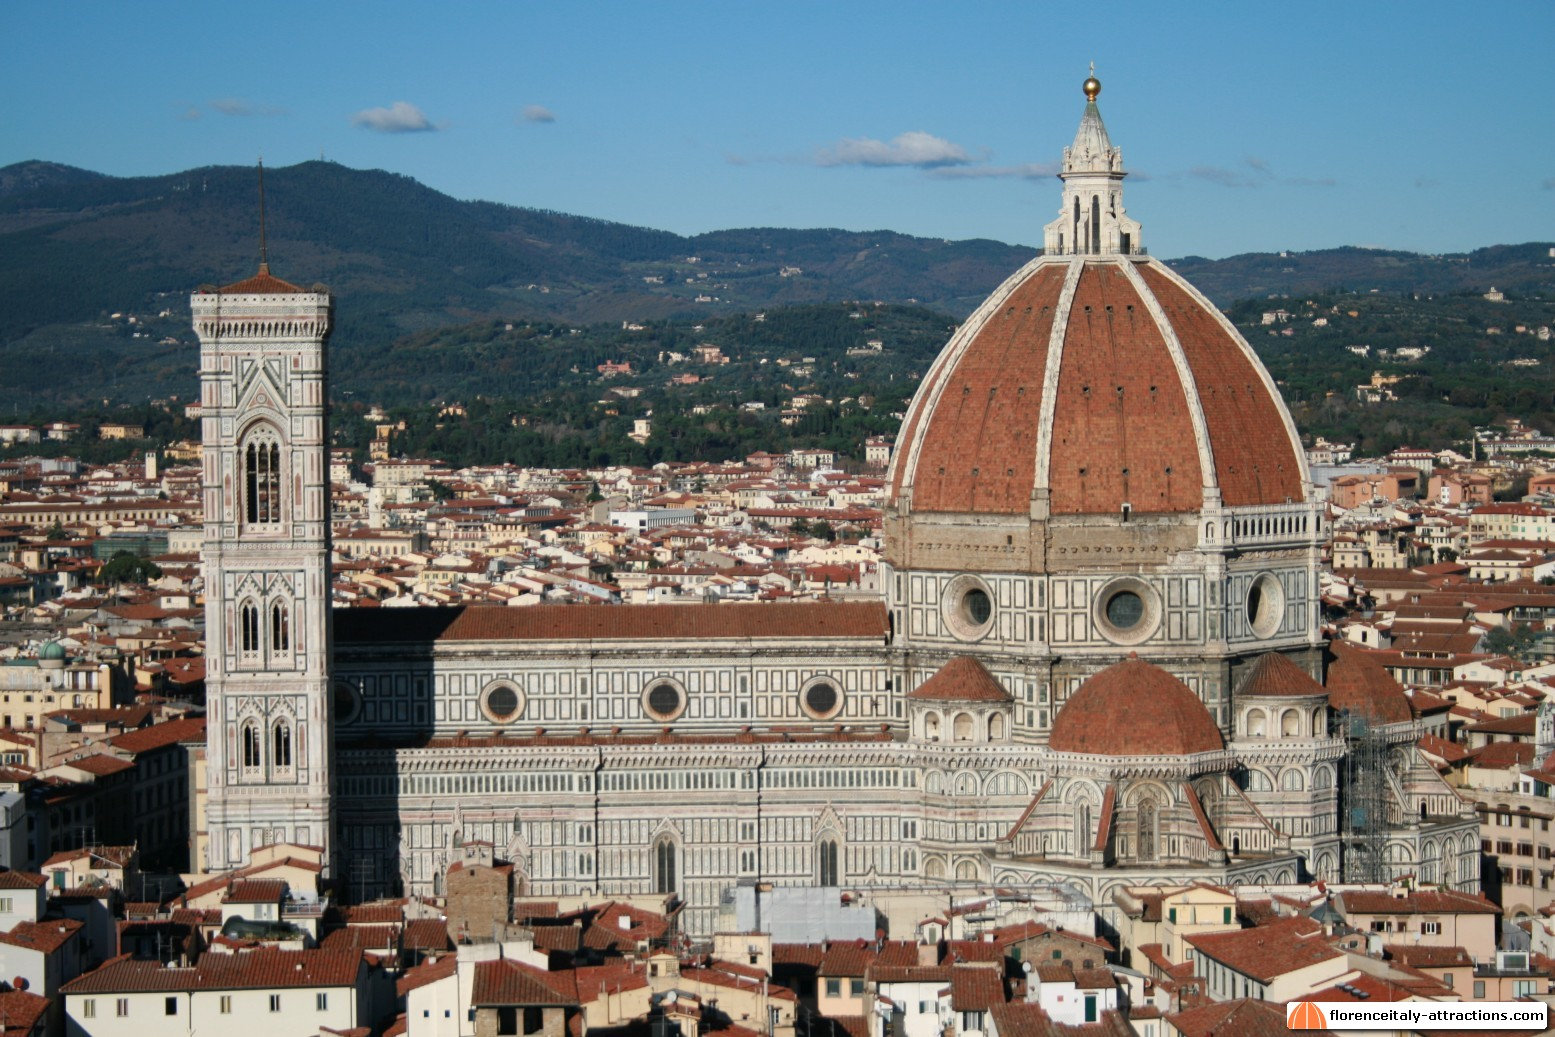
\includegraphics[width=.8\textwidth, height=.5\textwidth]{midias/foto.jpg}
			\\
			\textbf{\footnotesize Fonte: Elaborado pelo autor}
			\label{foto1}
		\end{center}
	
	\section{\esp Declaração de Figuras}\label{section:2.1}
		
			\begin{figure}[!ht]
				\setlength{\baselineskip}{\baselineskip} % Espacamento: simples
				\centering	
				\caption[\hspace{0.1cm} venus, cupid, Time and folly]{venus, cupid, Time and folly}
				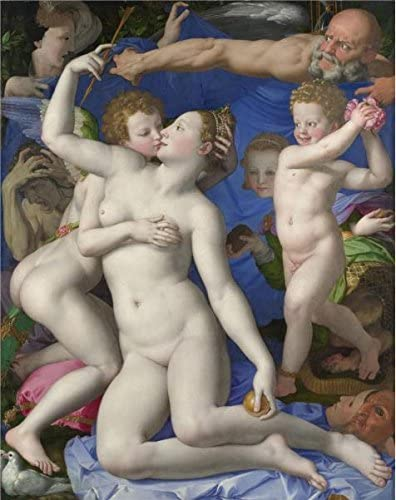
\includegraphics[width=.5\textwidth, height=.3\textwidth]{midias/figura.jpg}
				\\
				\textbf{\footnotesize Fonte: Agnolo Bronzino}
				\label{figura1}
			\end{figure}
		
			\begin{figure}[!ht]
				\setlength{\baselineskip}{\baselineskip} % Espacamento: simples
				\centering	
				\begin{tabular}{ c c }
				\caption[\hspace{0.1cm} Tabela com 4 figuras]{Tabela com 4 figuras}
					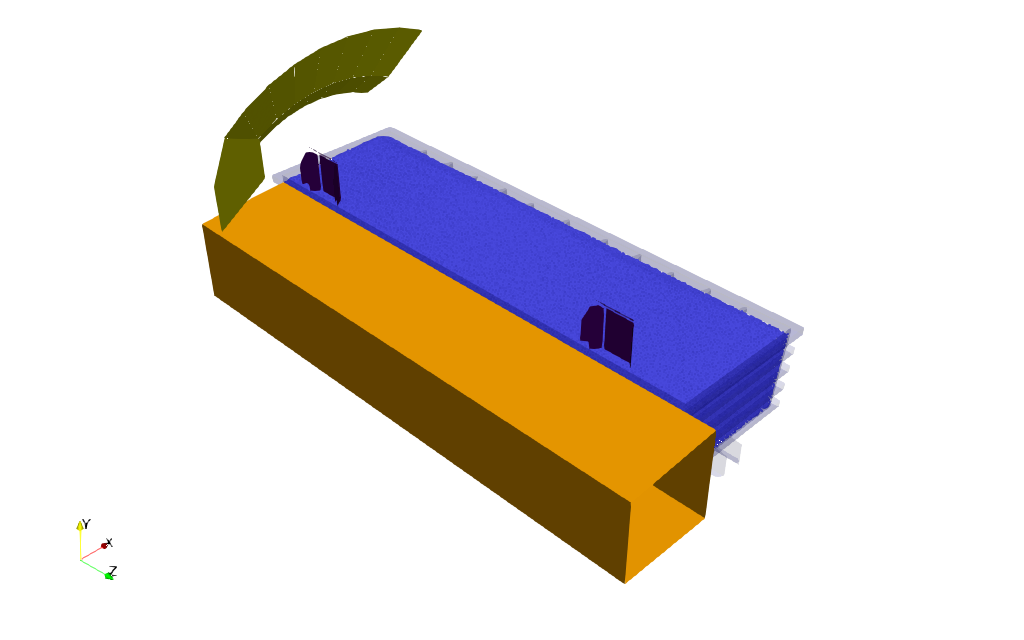
\includegraphics[width=.5\textwidth, height=.3\textwidth]{midias/figura6-1.png} &
					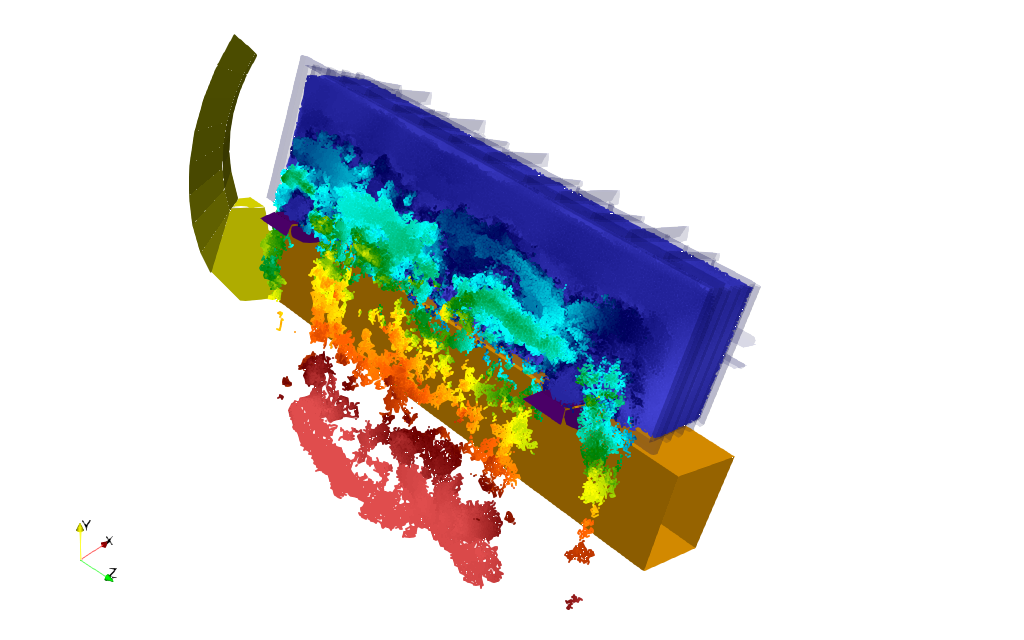
\includegraphics[width=.5\textwidth, height=.3\textwidth]{midias/figura6-2.png} \\
					a) \SI{0.0}{\second} & b) \SI{8.0}{\second} \\
					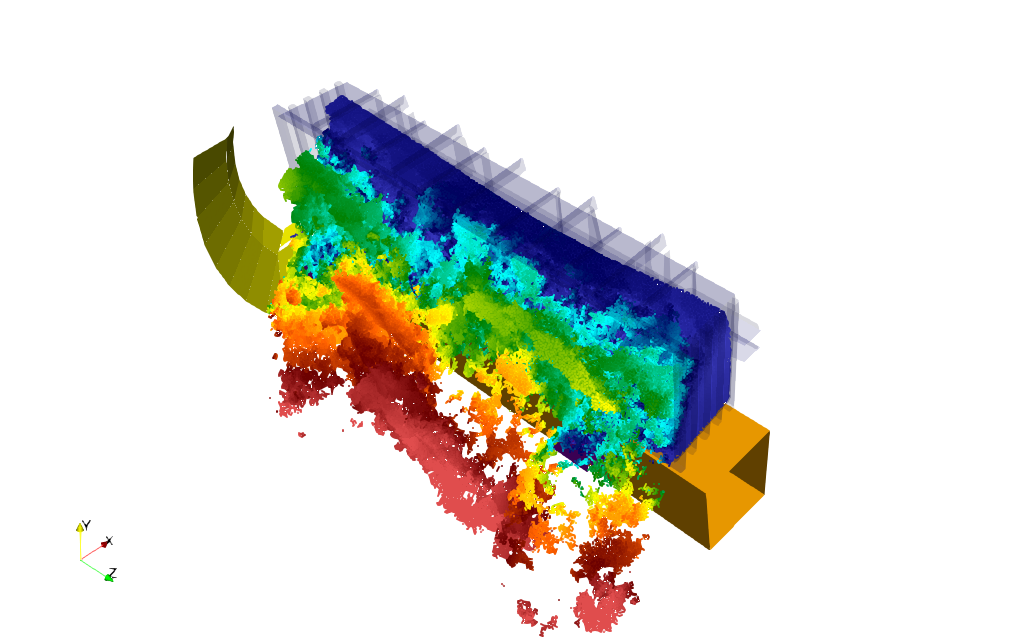
\includegraphics[width=.5\textwidth, height=.3\textwidth]{midias/figura6-3.png} &
					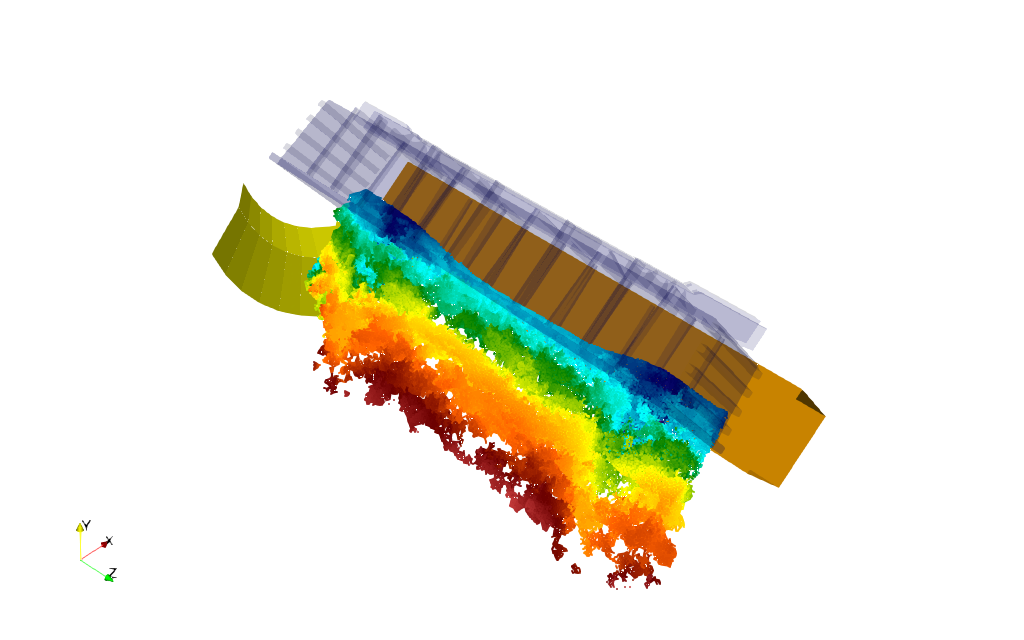
\includegraphics[width=.5\textwidth, height=.3\textwidth]{midias/figura6-4.png} \\
					c) \SI{10.0}{\second} & d) \SI{12.0}{\second} \\
				\end{tabular}
				\\
				\textbf{\footnotesize Fonte: Elaborado pelo autor}
				\label{fig2}
			\end{figure}
		
			\begin{figure}[!hb]
				\setlength{\baselineskip}{\baselineskip} % Espacamento: simples
				\centering
				\caption[\hspace{0.1cm} Figura 3D]{Figura 3D}
				\includemedia[
					width=0.8\linewidth,
					height=0.5\linewidth,
					%3Droo = 15000, % Radius of Orbit
					3Dcoo = 0 0 0, % Centrum of Orbit (Destino da camera)
					3Dc2c = -25000 25000 -25000, % Camera Center (Destino da camera)
					3Daac = 30, % Camera's aperture angle (Campo de visão)
					3Droll = -60, % Initial Rotation
					3Dlights=Headlamp,
					3Dmenu,
					activate=pagevisible,]
				{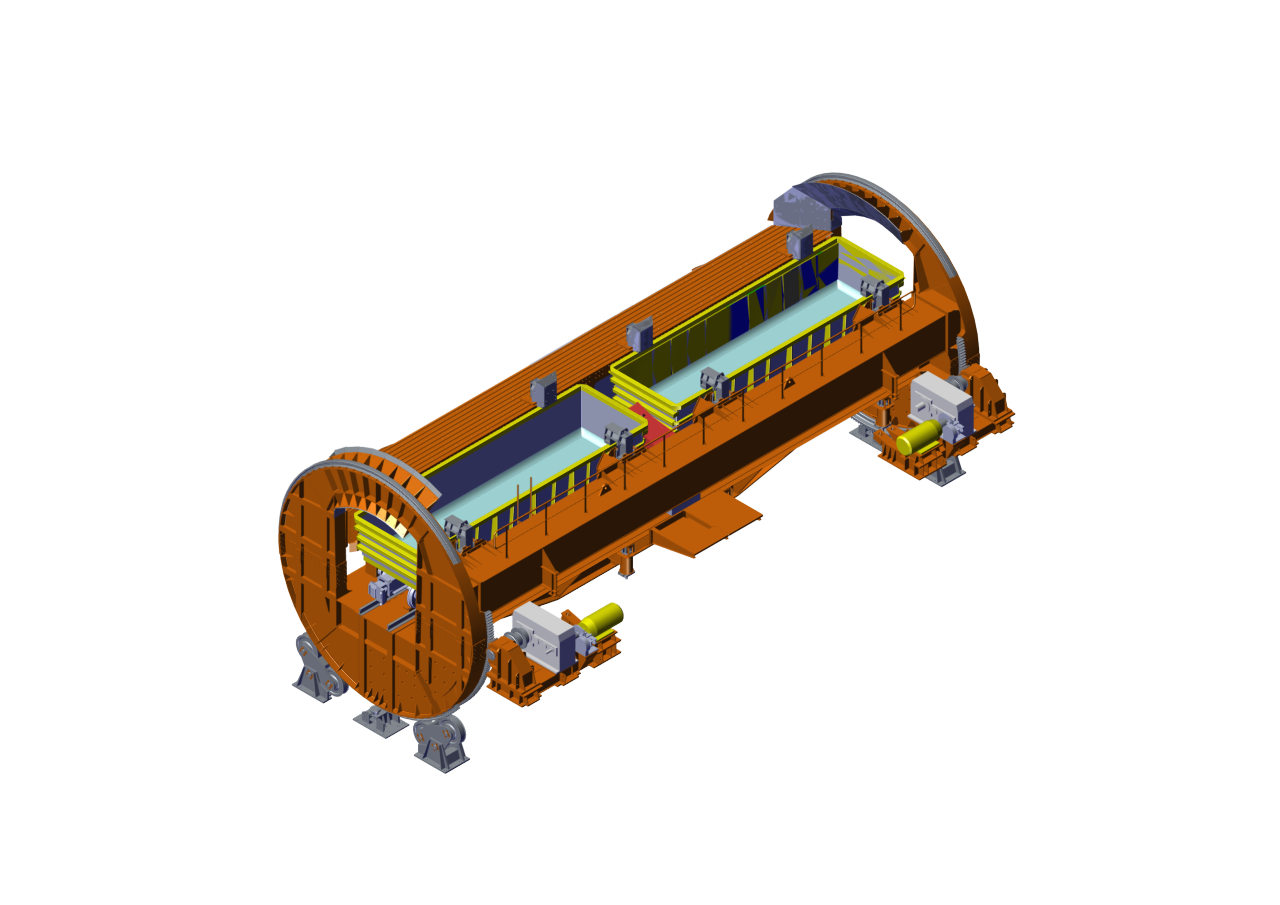
\includegraphics{midias/figura2.png}}
				{midias/figura2.u3d}
				\\
				\textbf{\footnotesize Fonte: Elaborado pelo autor}
				\label{fig14}
			\end{figure}
		
			\begin{figure}[!ht]
				\setlength{\baselineskip}{\baselineskip} % Espacamento: simples
				\centering
				\caption[\hspace{0.1cm} Figura com vídeo 1]{Figura com vídeo 1}
				\includemedia[
					%width=\linewidth,
					%height=0.375\linewidth,
					activate=pageopen,
					passcontext,
					transparent,
					addresource = midias/figura3.mp4,
					flashvars = {source=midias/figura3.mp4}
				]
				{
					\begin{tabular}{ c c }
						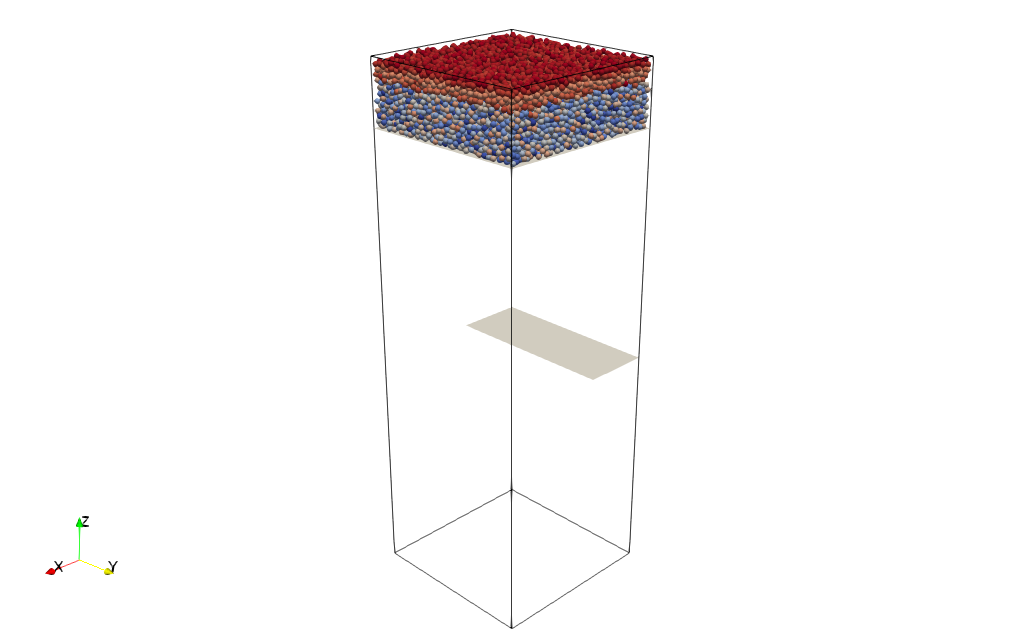
\includegraphics[width=0.5\textwidth, height=0.375\textwidth]{midias/figura3.png} &
						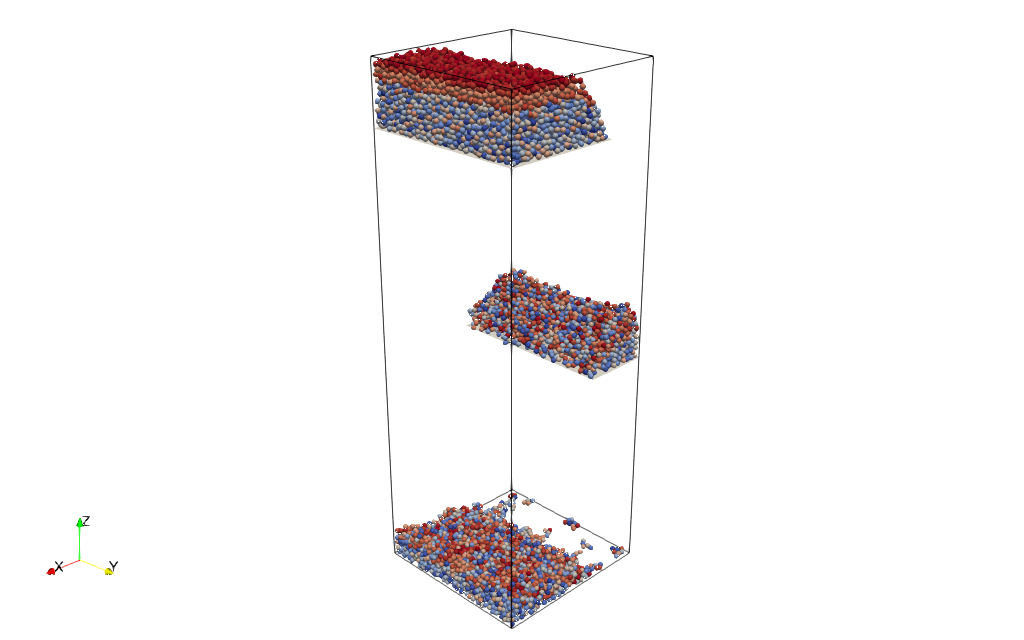
\includegraphics[width=0.5\textwidth, height=0.375\textwidth]{midias/figura4.png} \\
						a) Primeiro Passo de Tempo & b) Ultimo Passo de Tempo \\
					\end{tabular}
				}
				{VPlayer.swf}
				\\
				\textbf{\footnotesize Fonte: Elaborado pelo autor}
				\label{fig19}
			\end{figure}
			
			\begin{figure}[!ht]
				\setlength{\baselineskip}{\baselineskip} % Espacamento: simples
				\centering	
				\caption[\hspace{0.1cm} Figura com vídeo 2]{Figura com vídeo 2}
				\includemedia[
					width=0.8\linewidth,
					height=0.5\linewidth,
					activate=pageopen,
					passcontext,
					transparent,
					addresource=midias/figura5.mp4,
					flashvars={source=midias/figura5.mp4}
				]
				{ 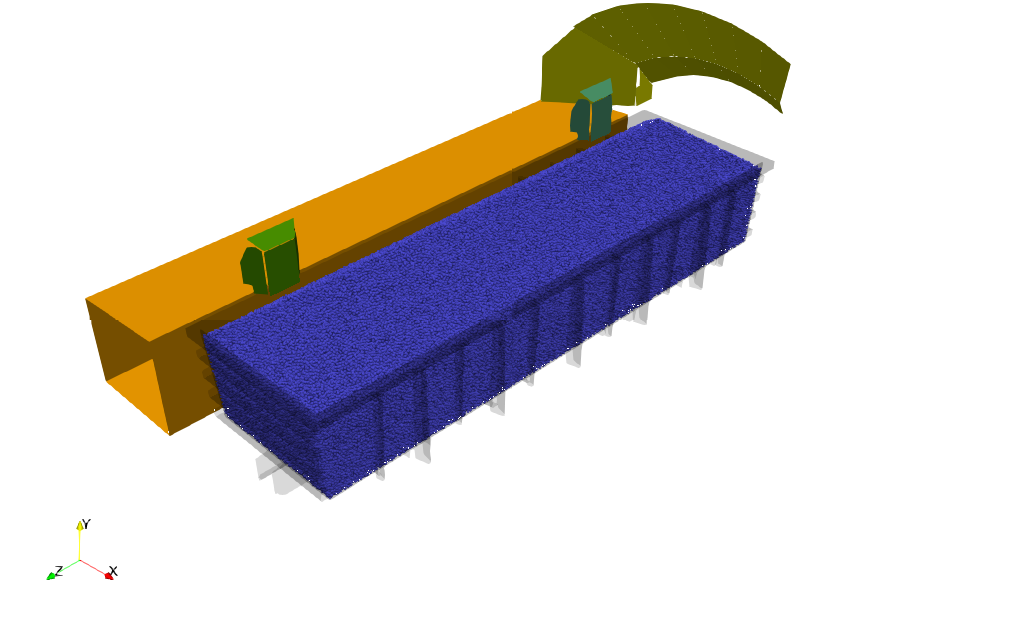
\includegraphics[width=0.8\textwidth, height=0.5\textwidth]{midias/figura5.png} }
				{VPlayer.swf}
				\\
				\textbf{\footnotesize Fonte: Elaborado pelo autor}
				\label{fig20}
			\end{figure}
			
	\section{\esp Declaração de Tabelas}\label{section:2.1}	
		
		\begin{table}[!ht]
			\centering
			\caption[\hspace{0.1cm} Relação Entre a Cor na Malha e a Espessura do Elemento de Placa]{Relação Entre a Cor na Malha e a Espessura do Elemento de Placa}
			\vspace{-0.3cm} % espaço entre titulo e tabela
			\begin{tabular}{c|c}
				\hline
				\textbf{Cor} & \textbf{Espessura do Elemento de Placa} \\
				\hline
					\cellcolor{cor1} & \SI[{scientific-notation = engineering}]{8.0}{\milli\meter} \\
					\cellcolor{cor2} & \SI[{scientific-notation = engineering}]{3.0}{\milli\meter} \\
					\cellcolor{cor3} & \SI[{scientific-notation = engineering}]{6.3}{\milli\meter} \\
					\cellcolor{cor4} & \SI[{scientific-notation = engineering}]{15.8}{\milli\meter} \\
					\cellcolor{cor5} & \SI[{scientific-notation = engineering}]{19.0}{\milli\meter} \\
					\cellcolor{cor6} & \SI[{scientific-notation = engineering}]{9.5}{\milli\meter} \\
					\cellcolor{cor7} & \SI[{scientific-notation = engineering}]{19.0}{\milli\meter} \\
					\cellcolor{cor8} & \SI[{scientific-notation = engineering}]{12.7}{\milli\meter} \\
					\cellcolor{cor9} & \SI[{scientific-notation = engineering}]{4.8}{\milli\meter} \\
					\cellcolor{cor10} & \SI[{scientific-notation = engineering}]{22.2}{\milli\meter} \\
					\cellcolor{cor11} & \SI[{scientific-notation = engineering}]{40.0}{\milli\meter} \\
					\cellcolor{cor12} & \SI[{scientific-notation = engineering}]{3.0}{\milli\meter} \\
				\hline
			\end{tabular}
			\\
			\small{\textbf{\footnotesize Fonte: Elaborado pelo autor}}
			\label{tab1}
		\end{table}
			
		\begin{table}[!ht]
			\centering
			\caption{\hspace{0.1cm} Somatório das Forças de Reação na Lateral da Caixa em Cada Passo de Tempo}
			\vspace{-0.3cm} % espaço entre titulo e tabela
			\begin{tabular}{c|c|c|c}
			  \hline
			  \textbf{Instante [0.2 s]} & \textbf{Força X [N]} & \textbf{Força Y [N]} & \textbf{Força Z [N]} \\
			  \hline

			  \SI[{scientific-notation = engineering, round-precision=2}]{+0.000E+00}{} & 
			  \SI[{scientific-notation = engineering, round-precision=2}]{-6.655E+00}{} & 
			  \SI[{scientific-notation = engineering, round-precision=2}]{+5.527E+01}{} & 
			  \SI[{scientific-notation = engineering, round-precision=2}]{+1.942E-01}{} \\

			  \SI[{scientific-notation = engineering, round-precision=2}]{+1.000E+00}{} &
			  \SI[{scientific-notation = engineering, round-precision=2}]{+1.872E+03}{} &
			  \SI[{scientific-notation = engineering, round-precision=2}]{+4.754E+04}{} &
			  \SI[{scientific-notation = engineering, round-precision=2}]{+1.778E+03}{} \\

			  \SI[{scientific-notation = engineering, round-precision=2}]{+2.000E+00}{} &
			  \SI[{scientific-notation = engineering, round-precision=2}]{+8.157E+03}{} &
			  \SI[{scientific-notation = engineering, round-precision=2}]{+3.409E+04}{} &
			  \SI[{scientific-notation = engineering, round-precision=2}]{+1.483E+03}{} \\

			  \SI[{scientific-notation = engineering, round-precision=2}]{3.000E+00}{} &
			  \SI[{scientific-notation = engineering, round-precision=2}]{1.726E+04}{} &
			  \SI[{scientific-notation = engineering, round-precision=2}]{4.410E+04}{} &
			  \SI[{scientific-notation = engineering, round-precision=2}]{1.305E+03}{} \\

			  \SI[{scientific-notation = engineering, round-precision=2}]{4.000E+00}{} &
			  \SI[{scientific-notation = engineering, round-precision=2}]{3.403E+04}{} &
			  \SI[{scientific-notation = engineering, round-precision=2}]{6.933E+04}{} &
			  \SI[{scientific-notation = engineering, round-precision=2}]{1.672E+03}{} \\

			  \SI[{scientific-notation = engineering, round-precision=2}]{5.000E+00}{} &
			  \SI[{scientific-notation = engineering, round-precision=2}]{3.046E+04}{} &
			  \SI[{scientific-notation = engineering, round-precision=2}]{6.032E+04}{} &
			  \SI[{scientific-notation = engineering, round-precision=2}]{1.763E+03}{} \\
			  \hline
			\end{tabular}
			\\
			\small{\textbf{\footnotesize Fonte: Elaborado pelo autor}}
			\label{tab2}
		\end{table}
			
		\begin{table}[!ht]
			\centering
			\caption{\hspace{0.1cm} Parâmetros de entrada usados na simulação}
			\vspace{-0.3cm} % espaço entre titulo e tabela
			\begin{tabular}{l|l}
				\hline
				\textbf{Propriedade} & \textbf{Valor} \\
				\hline
					Raio da partícula & \SI[{scientific-notation = engineering}]{20e-3}{\meter} \\
					Módulo de Young - Partícula & \SI[{scientific-notation = engineering}]{33e6}{\Pa} \\
					Módulo de Young - Parede & \SI[{scientific-notation = engineering}]{210e9}{\Pa} \\
					Coeficiente de Poisson - Partícula & \num{0.3} \\
					Coeficiente de Poisson - Parede & \num{0.3} \\
					Coeficiente de Restituição Partícula-Partícula & \num{0.15} \\
					Coeficiente de Restituição Partícula-Parede & \num{0.5} \\
					Massa Específica da Partícula & \SI[{scientific-notation = engineering}]{6242.4885608081559}{\kilogram \per \meter^3} \\
					Coeficiente de atrito estático partícula-partícula & \num{0.75112433653362509} \\
					Coeficiente de atrito estático partícula-parede & \num{0.72660908634539001} \\
					Coeficiente de resistência ao rolamento partícula-partícula & \num{0.056109958815042701} \\
					Coeficiente de resistência ao rolamento partícula-parede & \num{0.083343906361406012} \\
					Energia de coesão partícula-partícula & \SI[{scientific-notation = engineering}]{830483.5659099475}{\joule \per \meter^3} \\
					Energia de coesão partícula-parede & \SI[{scientific-notation = engineering}]{252798.56358366983}{\joule \per \meter^3} \\
				\hline
			\end{tabular}
			\\
			\small{\textbf{\footnotesize Fonte: Elaborado pelo autor}}
			\label{tab3}
		\end{table}
		
	\section{\esp Declaração de Gráficos}\label{section:2.1}
		
		\begin{grafico}
			\centering	
			\graficos{Velocidade Angular do Equipamento Durante o Descarregamento}
			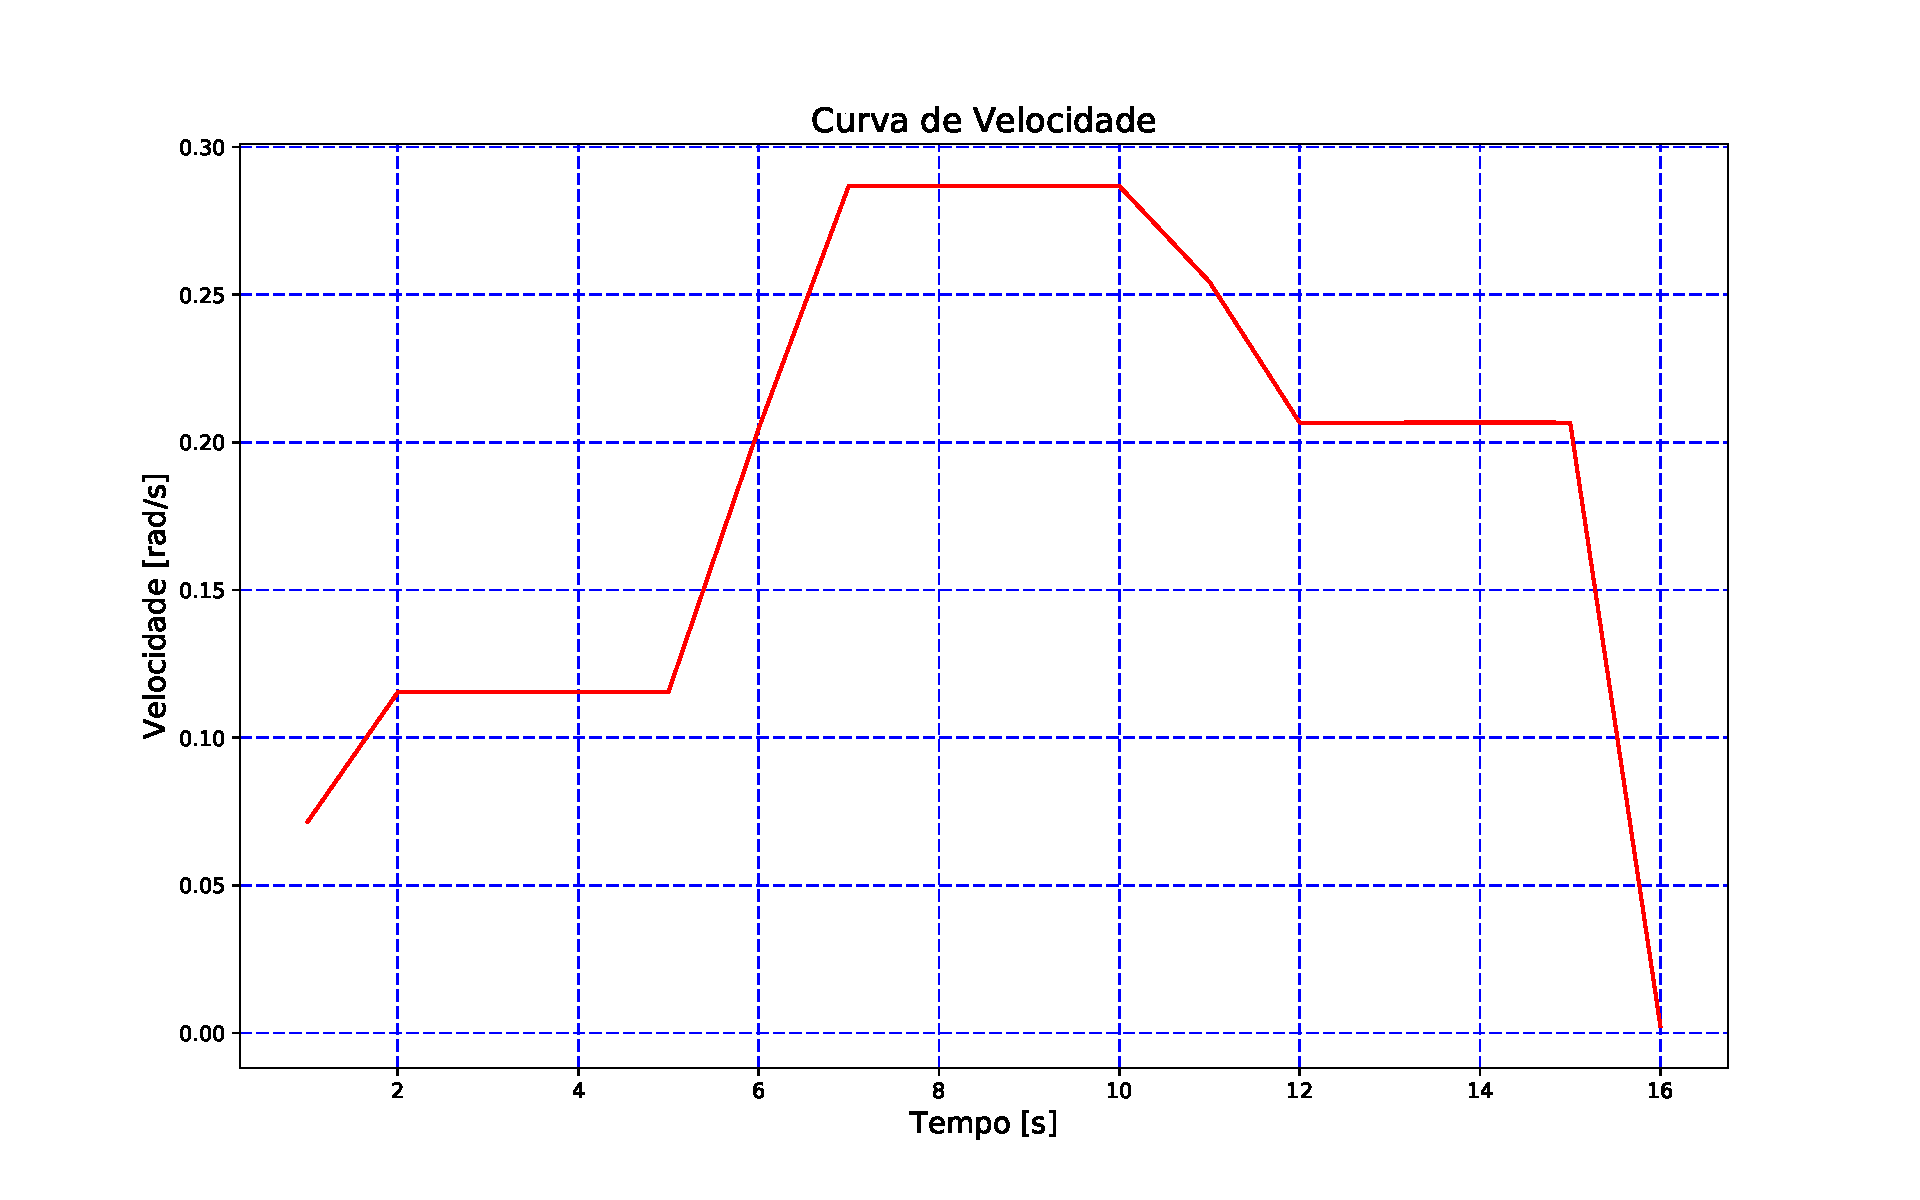
\includegraphics[width=.8\textwidth, height=.5\textwidth]{midias/grafico1.pdf}
			\\
			\textbf{\footnotesize Fonte: Elaborado pelo autor}
			\label{graf1}
		\end{grafico}
		
	
	\section{\esp Declaração de Siglas}\label{section:2.1}
		
		\sigla{MED}{Método dos Elementos Discretos}{1};
		\sigla{MEF}{Método dos Elementos Finitos}{1};
		\sigla{LAMMPS}{Large-scale Atomic/Molecular Massively Parallel Simulator}{1};
		\sigla{DFC}{Dinâmica dos fluidos computacional}{1};
		\sigla{LHS}{Latin HyperCube Sampling}{1};
		\sigla{STL}{StereoLithograph}{1};
		\sigla{CCDM}{Combined Continuum and Discrete Method}{1}.
	
	\section{\esp Declaração de Símbolos Matemáticos}\label{section:2.1}
	
		\simbolo{$ m_{i} $}{Massa da partícula}{1};
		\simbolo{$ \vec{v_{i}} $}{Velocidade de translação}{1};
		\simbolo{$ \vec{\omega_{i}} $}{Velocidade de rotação}{1};
		\simbolo{$ \vec{F_{i,j}^c} $}{Força de contato elástica}{1};
		\simbolo{$ \vec{F_{i,j}^d} $}{Força de amortecimento}{1};
		\simbolo{$ \vec{T_{i,j}} $}{Torque devido as forças tangenciais}{1};
		\simbolo{$ \vec{M_{i,j}} $}{Torque devido ao atrito de rolamento}{1};
		\simbolo{$ \vec{g} $}{Vetor gravidade}{1};
		\simbolo{$ \Delta t_c $}{Passo de tempo}{1};
		\simbolo{$ \bar{R} $}{ Média dos raios das partículas}{1};
		\simbolo{$ \rho $}{Densidade das partículas}{1};
		\simbolo{$ G $}{Módulo de cisalhamento das partículas}{1};
		\simbolo{$ \vec{F}_{c} $}{Força de contato total}{1};
		\simbolo{$ \vec{F}_{n} $}{Força de contato normal}{1};
		\simbolo{$ \vec{F}_{t} $}{Força de contato tangencial}{1};
		\simbolo{$ \vec{K}_n $}{Rigidez normal da mola}{1};
		\simbolo{$ \vec{N}_n $}{Coeficiente de amortecimento normal}{1};
		\simbolo{$ R_{eq} $}{Raio equivalente}{1};
		\simbolo{$ M_{eq} $}{Massa equivalente}{1};
		\simbolo{$ E_{eq} $}{Módulo de Young equivalente}{1};
		\simbolo{$ d_{n} $}{Sobreposição dos raios das partículas no ponto de contato}{1};
		\simbolo{$ v_{n} $}{Velocidade normal da colisão}{1};
		\simbolo{$ N_{n} $}{Coeficiente de amortecimento normal}{1}.
		\simbolo{ $ M_{A} $}{Massa da partícula A}{1};
		\simbolo{$ M_{B} $}{Massa da partícula B}{1}.
		\simbolo{$ \nu_{A} $}{Coeficiente de Poisson da partícula A}{1};
		\simbolo{$ \nu_{B} $}{Coeficiente de Poisson da partícula B}{1};
		\simbolo{$ E_{A} $}{Módulo de Young da partícula A}{1};
		\simbolo{$ E_{B} $}{Módulo de Young da partícula B}{1}.
		\simbolo{$ C_{fs} $}{Coeficiente de atrito estático}{1};
		\simbolo{$ v_{t} $}{Velocidade tangencial da colisão}{1};
		\simbolo{$ \vec{N_{t}} $}{Coeficiente de amortecimento tangencial}{1}.
		\simbolo{$ u_3 $}{Deslocamento em qualquer ponto da placa}{1};
		\simbolo{$ \bar{u_3} $}{Deslocamento em qualquer ponto da linha material}{1};
		\simbolo{$ x_1 $}{Posição no eixo $x_1$}{1};
		\simbolo{$ x_2 $}{Posição no eixo $x_2$}{1};
		\simbolo{$ x_3 $}{Posição no eixo $x_3$}{1}.
		\simbolo{$ \Phi_1 $}{Rotação da linha material em relação ao eixo $\bar{i_1}$}{1};
		\simbolo{$ \Phi_2 $}{Rotação da linha material em relação ao eixo $\bar{i_2}$}{1}.
		\simbolo{$ \epsilon_3 $}{Deformação na direção normal ao elemento}{1}
		\simbolo{$ \gamma_{13} $}{Deformação por cisalhamento no plano definido pelos eixos 1 e 3}{1}
		\simbolo{$ \gamma_{23} $}{Deformação por cisalhamento no plano definido pelos eixos 2 e 3}{1}
		\simbolo{$ \epsilon_1 $}{Deformação normal em relação ao eixo $x_1$}{1};
		\simbolo{$ \epsilon_2 $}{Deformação normal em relação ao eixo $x_2$}{1};
		\simbolo{$ \gamma_{12} $}{Deformação por cisalhamento no plano definido pelos eixos 1 e 2}{1}.
		\simbolo{\underline{$ \epsilon $}}{Matriz coluna das deformações no plano}{1}.
		\simbolo{\underline{\underline{S}}}{Matriz de permutação}{1}.
		\simbolo{\underline{N}}{Matriz coluna das forças no plano}{1}.
		\simbolo{\underline{$ \sigma $}}{Matriz coluna das tensões no plano}{1}.
		\simbolo{\underline{M}}{Matriz coluna dos momentos}{1}.
		\simbolo{$G$}{Modulo de cisalhamento}{1} definido por:
		\simbolo{\underline{\underline{C}}}{Matriz de rigidez para o estado plano de tensões}{1}.
		\simbolo{$ h $}{Espessura da placa}{1}.
		\simbolo{\underline{\underline{A}}}{Matriz de rigidez do plano médio}{1} definida por:
		\simbolo{\underline{\underline{D}}}{Matriz de rigidez a flexão para material homogêneo e isotrópico}{1}
		\simbolo{$ \nu $}{Coeficiente de poisson}{1}.
		\simbolo{$ R_{A} $}{Raio da partícula A}{1};
		\simbolo{$ R_{B} $}{Raio da partícula B}{1}.
		\simbolo{$ R_{r} $}{Raio de rolamento}{1}; \simbolo{$ \mu_{r} $}{Coeficiente de resistência ao rolamento}{1};
		\simbolo{$ F_{n} $}{Força de contato normal}{1}.
		\simbolo{$ \eta_{r} $}{Razão de amortecimento viscoso de rolamento}{1};
		\simbolo{$ C^{crit}_{r} $}{Constante critica de amortecimento viscoso}{1}
	
	\section{\esp Declaração de Listas}\label{section:2.1}
	
		\begin{itemize}
			\item{Venus, Cupid, Folly and Time;}
			\item{Holy Family;}
			\item{Deposition of Christ.}
		\end{itemize}
		\begin{itemize}
			\item{\textbf{Seis equações de deformação-deslocamento}:}
			\begin{itemize}
				\item{Três equações definem a deformação no plano médio em relação aos deslocamentos no plano médio; (equações \ref{eq2.67})}
				\item{Três equações definem a curvatura da placa em relação aos deslocamentos transversais. (equação \ref{eq2.68})}
			\end{itemize}

			\item{\textbf{Cinco equações de equilíbrio}:}
			\begin{itemize}
				\item{Duas equações expressam as condições de equilíbrio para as forças no plano; (equações \ref{eq2.88} e \ref{eq2.89})}
				\item{Uma equação expressa a condição de equilíbrio para as forças verticais; (equação \ref{eq2.90})}
				\item{Duas equações expressam a condição de equilíbrio para os momentos. (equações \ref{eq2.91} e \ref{eq2.92})}
			\end{itemize}

			\item{\textbf{Seis leis constitutivas}:}
			\begin{itemize}
				\item{Três equações que relacionam as forças no plano e as deformações no plano médio; (equação \ref{eq2.107})}
				\item{Três equações que relacionam os momentos fletores e as curvaturas; (equação \ref{eq2.110})}
			\end{itemize}
		\end{itemize}
		\begin{enumerate}
			\item{\label{item1} A linha normal ao plano médio (linha material) é infinitamente rígida em seu comprimento;}
			\item{\label{item2} Durante a deformação, a linha material se mantém reta e normal ao plano médio deformado da placa;}
			\item{\label{item3} A linha material se mantém normal ao plano médio deformado.}
		\end{enumerate}
          
		
		
	\section{\esp Exemplos de Citações}\label{section:2.1}
	
		Citação direta tipo miscelania:
			To explain all nature is too difficult a task for any one man or even for any one age. 'Tis much better to do a little with certainty, and leave the rest for others that come after you, than to explain all things by conjecture without making sure of anything. \citeAutorAno{Newton_1704}.
			
		Citação direta tipo artigo:
			Segundo \citeAutorAno{Rackl_2017} o processo de calibração consiste em variar os parâmetros desconhecidos até que seja atingida uma correspondência satisfatória entre os resultados simulados e os valores medidos em experimentos físicos.
			
		Citação direta tipo livro:
			Segundo \citeAutorAno{Bauchau_2012}, placa ou casca é definida como um sólido tridimensional em que uma das dimensões é muito menor que as demais.
			
		Citação Direta tipo dissertação de mestrado:
			Estes métodos numéricos de integração no tempo são divididos e conceituados como explícitos ou implícitos.  \cite{Mendes_2012}.
			
		Citação direta tipo tese de doutorado:
			No trabalho de \citeAutorAno{Johnstone} o autor desenvolveu uma metodologia para a calibração \sigla{MED}{}{0} de grãos utilizando a resposta extraída de experimentos físicos.
			
		Citação direta tipo manual:
			Conforme \citeAutorAno{Tomas_2013}, este elemento deve ser empregado em estudos com pequeno deslocamento e deformação, de elementos estruturais curvos ou planos.
			
		Citação direta tipo anais de congresso:
			No trabalho de \citeAutorAno{Parteli_2013} é proposto um algoritmo para modelar a dinâmica envolvida nas partículas utilizadas no processo de impressão 3D.
			
		Citação indireta:
			Nas simulações MED é assumido que toda a energia é transferida via ondas de Rayleighsem grandes prejuízos, visto que a diferença entre as velocidades das ondas de Rayleigh e asondas distorcionais é muito pequena e a energia devido as ondas de dilatação também é pequenae pode ser desprezada. Além disso o tempo médio da chegada da onda de Rayleigh em qualquercontato é a mesma, independente da localização do ponto de contato. \cite{Rackl_2017}.
			
		Citação de link:
			O \href{https://github.com/CFDEMproject/LIGGGHTS-PUBLIC}{LIGGGHTS®-PUBLIC 3.7.1} possibilita a simulação de diversas vertentes da engenharia que utilizam materiais granulares.
			
		Citação de apêndice:
			Os detalhes dos algoritmos desenvolvidos podem ser encontrados nos Apêndices \ref{app:A}.
			
		Citação de gráfico:
			O Gráfico \ref{graf1} relaciona a densidade efetiva da partícula no eixo horizontal e a densidade aparente de reposta do programa no eixo vertical.
			
		Citação de símbolo grego:
			O termo $ \beta $ pode ser obtido por:
			A minimização do resíduo se dá pela integração da multiplicação de $ R $ por uma função de ponderação $ \psi $ no domínio $ \Gamma $, tendo em ressalto que o resultado deverá ser nulo.
			
		Citação de figura:
			A Figura \ref{figura1} apresenta o diagrama de forças.
			
		Citação de equação:
			As equações que definem a força normal, rigidez normal da mola e amortecimento normal são definidas por \ref{eq2.15}, \ref{eq2.16} e \ref{eq2.17} respectivamente.
			
		Citação de símbolo matemático:
			E o \simbolo{$ \vec{N_{n}} $}{Coeficiente de amortecimento normal}{1} por:
			A \simbolo{$ M_{r} $}{Resistência de rolamento total}{2} é definida por:
			A primeira componente da resistência ao rolamento total é o \simbolo{$ \Delta M^k_{r} $}{Incremento no torque}{2}.
			Onde \simbolo{$ \Delta \theta_{r} $}{Rotação relativa entre duas partículas}{1}.
			A \simbolo{\underline{$ \epsilon_0 $}}{Matriz de deformações no plano}{2} pode ser definida por:

	\section{\esp Declaração de Números no Texto}\label{section:2.1}

		Número génerico: \num{10e-6}.
		
		Porcentagem: \SI{7}{\%}.
		
		Segundos com 6 casas decimais: \SI[{round-precision=6}]{0.00015640340337823129}{\second}.
    
	\section{\esp Exemplo de Equação no Texto}\label{section:2.1}
			
		Ao utilizar o Método de Newmark um teste de estabilidade pode ser realizado, ou seja, para que ele seja considerado estável, a condição estabelecida pela relação $ \beta \leq \frac{1}{2} \leq \alpha $ quando $ \Delta t \leq \frac{\sqrt{2}}{w_{max} \sqrt{ \alpha - 2 \beta}} $ deve ser verdadeira. Consequentemente a convergência do método pode ser garantida se a matriz de rigidez apresentar simetria e todos os valores forem positivos.
			
	\section{\esp Exemplo de Equações}\label{section:2.1}
		
		\begin{equation}\label{eq2.9}
			m_{i}\frac{d\vec{v_{i}}}{dt} = \sum_{j=1}^{n}  \left( \vec{F^c_{i,j}}+\vec{F^d_{i,j}} \right) + m_{i}*\vec{g}
		\end{equation}

		\begin{equation}\label{eq2.10}
			I_{i}\frac{d\vec{\omega_{i}}}{dt} = \sum_{j=1}^{n}(\vec{T_{i,j}}+\vec{M_{i,j}})
		\end{equation}
		
		\begin{equation}\label{eq2.11}
			\Delta t_c = \frac{\pi \bar{R}}{\beta} \sqrt{\frac{\rho}{G}}
		\end{equation}
		
		\begin{equation}\label{2.12}
			(2 - \beta^2)^4 = 16*(1-\beta^2)*\left[ 1 - \beta^2* \left( \frac{1 - 2*\nu}{2*(1-\nu} \right) \right]
		\end{equation}
		
		\begin{equation}\label{2.13}
			\beta = 0.8766 + 0.163 \nu
		\end{equation}
		
		\begin{equation}\label{eq2.14}
				\vec{F}_{c} = \vec{F}_{n} + \vec{F}_{t}
		\end{equation}
		
		\begin{equation}\label{eq2.15}
					\vec{F}_{n} = -K_n d_n - N_n v_n
		\end{equation}
		
		\begin{equation}\label{eq2.16}
				\vec{K}_{n} = \frac{4}{3}E_{eq}\sqrt{d_{n}R_{eq}}
		\end{equation}
		
		\begin{equation}\label{eq2.17}
				\vec{N}_{n} = \sqrt{(5K_{n}M_{eq})N_{n,damp}}
		\end{equation}
		
		\begin{equation}
				\frac{1}{R_{eq}} = \frac{1}{R_{A}} + \frac{1}{R_{B}}
		\end{equation}
		
		\begin{equation}
				\frac{1}{M_{eq}} = \frac{1}{M_{A}} + \frac{1}{M_{B}}
		\end{equation}
		
		\begin{equation}
				\frac{1}{E_{eq}} = \frac{1 - \nu^{2}_{A}}{E_{A}} + \frac{1 - \nu^{2}_{B}}{E_{B}}
		\end{equation}
		
		\begin{equation}
				\vec{F}_{t} = 
				\begin{cases}
						K_{t} d_{t} - N_{t}v_{t} &, \text{se} \left| K_{t} d_{t} \right| < \left| K_{n} d_{n} \right| C_{fs} \\
						\frac{ \left| K_{n} d_{n} \right| C_{fs} d_{t} }{ \left| d_{t} \right| } &, \text{se} \left| K_{t} d_{t} \right| \geq \left| K_{n} d_{n} \right| C_{fs}
				\end{cases}
		\end{equation}
		
		\begin{equation}
				\vec{K}_{t} = 8 G_{eq} \sqrt{d_t R_{eq}}
		\end{equation}
		
		\begin{equation}
				\vec{N}_{t} = \sqrt{5 K_t Meq} N_t
		\end{equation}
		
		\begin{equation}
				\vec{N}_{t} = 
				\begin{cases}
						1, & \text{se } C_{rest} = 0 \\
						\frac{ -ln(C_{n,rest}) }{ \sqrt{\Pi^2 + ln(C_{n,rest})^2 } }, & \text{Caso contrário}
				\end{cases}
		\end{equation}
		
		\begin{equation}
			\frac{1}{G_{eq}} = \frac{2(2 - v_A)(1 + v_A)}{E_A} + \frac{2(2 - v_B)(1 + v_B)}{E_B}
		\end{equation}
		
		\begin{equation}
			M_{r} = M^k_{r} + M^d_{r}
		\end{equation}
		
		\begin{equation}
			\Delta M^k_{r} = -k_{r} \Delta \theta_{r}
		\end{equation}

		\begin{equation}
				\begin{cases}
					M^k_{r,t+\Delta t} = M^k_{r,t} + \Delta M^k_{r} \\
					\left| M^k_{r,t + \Delta t} \right| \leq M^m_{r}
				\end{cases}
		\end{equation}
		
		\begin{equation}
			M^m_{r} = \mu_{r} R_{r} F_{n}
		\end{equation}

		\begin{equation}
			\theta^m_{r} = \frac{\mu_{r}}{2J_{n}}
		\end{equation}

		\begin{equation}
			k_{r} = \frac{\mu_{r}R_{r}F_{n}}{\theta^m_{r}}
		\end{equation}
		
		\begin{equation}
				M^d_{r,t + \Delta t}
				= 
				\begin{cases}
					-C_{r}\dot{\theta_{r}} & \text{se} \left| M^k_{r,t+ \Delta t} \right| < M^m_{r} \\
					-fC_{r}\dot{\theta_{r}} & \text{se} \left| M^k_{r,t + \Delta t} \right| = M^m_{r}
				\end{cases}
		\end{equation}
		
		\begin{equation}
			C_{r} = \eta_{r}C^{crit}_{r}
		\end{equation}

		\begin{equation}
			c^{crit}_{r} = 2\sqrt{I_{r}k_{r}}
		\end{equation}

		\begin{equation}
			\frac{1}{I_{r}} = \frac{1}{I_{i}+m_{i}r^2_{i}} + \frac{1}{I_{j}+m_{j}r^2_{j}}
		\end{equation}
		
		\begin{equation}\label{eq:2.9}
			\int_{V}^{} f dV = \sum_{i=1}^{n} \int_{V_{i}}^{} f dV
		\end{equation}
		
		\begin{equation}\label{eq:2.10}
			V = \sum_{i=1}^{n} V_{i}
		\end{equation}

		\begin{equation}
			F = \sum_{n = 1}^{N} A_{n} \phi_{n}
		\end{equation}
	 
		\begin{equation} \label{eq2.39}
			\int_{ \Gamma} R \Psi_j dt =0, para j=1 … N
		\end{equation}

		\begin{equation} \label{eq:2.12}
			Erro = exata - aproximada
		\end{equation}
	   
		\begin{equation} \label{eq:2.14}
			\langle r, \phi_i \rangle = \int_{ D} r(x) \phi_i(x) dx = 0
		\end{equation}
		
		\begin{equation}\label{eq2.42}
		  \int_{a}^{b} \Phi_{i} \Re_{i} dy
		\end{equation}

		\begin{equation} \label{eq:2.16}
		  \psi_{j} = \phi_{j}
		\end{equation}

		\begin{equation} \label{eq:2.17}
		  \int_{a}^{b} \phi_{j} \Re_{i}  dy, \text{para} j = 1 ... N
		\end{equation}

		\begin{equation}\label{eq2.45}
			\underaccent{\bar}{u}(t_{0} + \epsilon)
			\approx
			\underaccent{\bar}{u}(t_{0})
			+\dot{\underaccent{\bar}{u}}(t_{0}) \epsilon 
			+\ddot{\underaccent{\bar}{u}}(t_{0}) \frac{\epsilon^2}{2}
			+\dddot{\underaccent{\bar}{\bar{u}}}(t_{0}) \frac{\epsilon^3}{6}
		\end{equation}
		
		\begin{equation} \label{eq2.46}
			\dot{\underaccent{\bar}{u}}(t_{0} + \epsilon)
			\approx
			\dot{\underaccent{\bar}{u}}(t_{0})
			+\ddot{\underaccent{\bar}{u}}(t_{0}) \epsilon 
			+\dddot{\underaccent{\bar}{u}}(t_{0}) \frac{\epsilon^2}{2}
		\end{equation}
		
		\begin{equation}
			\underaccent{\bar}{u}_{t + \Delta t}
			=
			\underaccent{\bar}{u}_t
			+\dot{\underaccent{\bar}{u}}_t \Delta t
			+\ddot{\underaccent{\bar}{u}} \frac{\Delta t^2}{2}
						+\beta \dddot{\underaccent{\bar}{u{t}}}_{t} \Delta t^3
		\end{equation}
		
		\begin{equation}
			\dot{\underaccent{\bar}{u}}_{t + \Delta t} =
			\dot{\underaccent{\bar}{u}}_t
			+\ddot{\underaccent{\bar}{u}}_t \Delta t
			+\alpha \dddot{\underaccent{\bar}{u}}_t \Delta t^2
		\end{equation}
		
		\begin{equation} \label{eq:2.15}
			\dddot{\underaccent{\bar}{u}}_{t}
			=
			\frac{\ddot{\underaccent{\bar}{u}}_{t  + \Delta t} - \ddot{\underaccent{\bar}{u}}_t}{ \Delta t }
		\end{equation}
		
		\begin{equation} \label{eq2.50}
			\underaccent{\bar}{u}_{t + \Delta t}
			=
			\underaccent{\bar}{u}_{t}
			+ \dot{\underaccent{\bar}{u}}_{t} \Delta t
			+ \left( \frac{1}{2} - \beta \right) \Delta t^2 \ddot{\underaccent{\bar}{u}}_{t}
			+ \beta \Delta t^2 \ddot{\underaccent{\bar}{u}}_{t + \Delta t}
		\end{equation}

		\begin{equation} \label{eq2.51}
			\dot{\underaccent{\bar}{u}}_{t + \Delta t}
			=
			\dot{\underaccent{\bar}{u}}_{t}
			+( 1 - \alpha) \Delta \ddot{\underaccent{\bar}{u}}_{t}
			+ \alpha \Delta t \ddot{\underaccent{\bar}{u}}_{t}
		\end{equation}
		 
		\begin{equation} \label{eq:2.18}
			\underaccent{\bar}{m} \ddot{\underaccent{\bar}{u}}_{t + \Delta t}
			\underaccent{\bar}{c} \dot{\underaccent{\bar}{u}}_{t + \Delta t}
			\underaccent{\bar}{k} \dot{\underaccent{\bar}{u}}_{t + \Delta t}
			=
			\underaccent{\bar}{f}_{t + \Delta t}
		\end{equation}
		
		\begin{equation}
		  u_3(x_1; x_2; x_3) = \bar{u_3}(x_1, x_2)
		\end{equation}

		\begin{equation}
		   u_1(x_1, x_2, x_3) = \bar{u_3}(x_1, x_2) + x_3 \Phi_2(x_1, x_2)
		\end{equation}
		   
		\begin{equation}
		   u_2(x_1, x_2, x_3) = \bar{u_2}(x_1, x_2) - x_3 \Phi_1(x_1, x_2)
		\end{equation}

		\begin{equation}
		  \Phi_1 = \frac{\partial \bar{u_3}}{\partial x_2}
		\end{equation}

		\begin{equation}
		  \Phi_2 = - \frac{\partial \bar{u_3}}{\partial x_1}
		\end{equation}

		\begin{equation}
		  u_1(x_1, x_2, x_3) = \bar{u_1}(x_1, x_2) - x_3 \frac{\partial \bar{u_3}}{x_1}
		\end{equation}

		\begin{equation}
		  u_2(x_1, x_2, x_3) = \bar{u_2}(x_1, x_2) - x_3 \frac{\partial \bar{u_3}}{x_2}
		\end{equation}

		\begin{equation}
		  u_3(x_1, x_2, x_3) = \bar{u_3}(x_1, x_2)
		\end{equation}

		\begin{equation}
		  \epsilon_3 = \frac{\partial u_3}{\partial x_3} = 0
		\end{equation}

		\begin{equation}
		  \gamma_{13} = \frac{\partial u_1}{\partial x_3} + \frac{\partial u_3}{\partial x_1} = - \frac{\partial \bar{x_3}}{\partial x_1} + \frac{\partial \bar{u_3}}{\partial x_1} = 0
		\end{equation}

		\begin{equation}
		  \gamma_{23} = \frac{\partial u_2}{\partial x_3} + \frac{\partial{u_3}}{\partial{x_2}} = - \frac{\partial \bar{x_3}}{\partial{x_2}
		  } + \frac{\partial{\bar{u_3}}}{\partial{x_2}} = 0
		\end{equation}

		\begin{equation}
		  \epsilon_1 = \frac{\partial{u_1}}{\partial{x_1}} = \frac{\partial{\bar{u_1}}}{\partial{x_1}} - x_3 \frac{\partial^2 \bar{u_3}}{\partial{x_1}^2}
		\end{equation}
		  
		\begin{equation}
		  \epsilon_2 = \frac{\partial{u_2}}{\partial{x_2}} = \frac{\partial{\bar{u_2}}}{\partial{x_2}} - x_3 \frac{\partial^2 \bar{u_3}}{\partial{x_2}^2},
		\end{equation}

		\begin{equation}
		  \gamma_{12} = \frac{\partial{u_1}}{\partial{x_2}} + \frac{\partial{u_2}}{\partial{x_1}} = \frac{\partial{\bar{u_1}}}{\partial{x_2}} + \frac{\partial{\bar{u_2}}}{\partial{x_1}} - 2x_3\frac{\partial^2 \bar{u_3}}{\partial{x_1}\partial{x_2}}
		\end{equation}

		\begin{equation}\label{eq2.67}
			\underline{\epsilon_0}
			=
			\left\{ 
			  \frac{\partial{\bar{u_1}}}{x_1}, \frac{\partial{\bar{u_2}}}{\partial{x_2}}, \frac{\partial{\bar{u_1}}}{\partial{x_2}}
			  + \frac{\partial{\bar{u_2}}}{\partial{x_1}}
			\right\}^T
			=
			\left\{
			  \epsilon_1, \epsilon_2, \epsilon_{12}
			\right\}^T
		\end{equation}
		  
		\begin{equation}\label{eq2.68}
			\underline{\kappa}
			=
			\left\{
			  \frac{\partial^2 \bar{u_3}}{\partial{x_2}^2},
			  - \frac{\partial^2 \bar{u_3}}{\partial{x_1}^2},
			  2 \frac{\partial^2 \bar{u_3}}{\partial{x_1}\partial{x_2}}
			\right\}^T
			=
			\left\{ 
			  \kappa_2, \kappa_2, \kappa_{12}
			\right\}^T
		\end{equation}
		  
		\begin{equation}
		  \epsilon_1 = \epsilon_1 + x_3 \kappa_2
		\end{equation}

		\begin{equation}
		  \epsilon_2 = \epsilon_2 + x_3 \kappa_1
		\end{equation}

		\begin{equation}
		  \gamma_{12} = \epsilon_{12} + x_3 \kappa_{12}
		\end{equation}
		 
		\begin{equation}\label{eq:2.56}
			\underline{\epsilon} = \underline{\epsilon_0} + x_3 \underline{\underline{S}} \underline{\kappa}
		\end{equation}

		\begin{equation}\label{eq:2.57}
			\underline{\epsilon} = \left\{ \epsilon_1, \epsilon_2, \gamma_{12} \right\} ^T
		\end{equation}

		\begin{equation}
			\underline{\underline{S}}
			=
			\begin{vmatrix}
				0 & 1 & 0 \\
				-1 & 0 & 0 \\
				0 & 0 & -1
			\end{vmatrix}
		\end{equation}
		
		\begin{equation}
		  N_1(x_1,x_2) = \int_h \sigma_1 dx_3
		\end{equation}
		\begin{equation}
		  N_2(x_1,x_2) = \int_h \sigma_2 dx_3
		\end{equation}
		\begin{equation}
		  N_{12}(x_1,x_2) = \int_h \tau_{12} dx_3
		\end{equation}

		\begin{equation}
		  \underline{N} = \int_h \underline{\sigma} dx_3
		\end{equation}

		\begin{equation}\label{eq:2.62}
		  \underline{N} = \left\{ N_1, N_2, N_{12} \right\}^T
		\end{equation}

		\begin{equation}\label{eq:2.64}
		  \underline{\sigma} = \left\{ \sigma_1, \sigma_2, \sigma_3 \right\}^T
		\end{equation}

		\begin{equation}
		  Q_1(x_1,x_2) = \int_h \tau_{13} dx_3
		\end{equation}

		\begin{equation}
		  Q_2(x_1,x_2) = \int_h \tau_{23} dx_3
		\end{equation}

		\begin{equation}
		  M_1(x_1,x_2) = -\int_h x_3 \sigma_2 dx_3
		\end{equation}

		\begin{equation}
		  M_2(x_1,x_2) = \int_h x_3 \sigma_1 dx_3
		\end{equation}

		\begin{equation}
		  M_{12}(x_1,x_2) = -\int_h x_3 \tau_{12} dx_3
		\end{equation}

		\begin{equation}
		  \underline{M} = \underline{\underline{S}}^T \int_h \underline{\sigma} x_3 dx_3
		\end{equation}

		\begin{equation}
		  \underline{M} = \left\{ M_1, M_2, M_{12} \right\}^T
		\end{equation}

		\begin{equation}\label{eq2.88}
		  \frac{\partial N_1}{\partial x_1} + \frac{\partial N_{12}}{\partial x_2} = -p_1
		\end{equation}

		\begin{equation}\label{eq2.89}
		  \frac{\partial N_{12}}{\partial x_1} + \frac{\partial N_{2}}{\partial x_2} = -p_2
		\end{equation}

		\begin{equation}\label{eq2.90}
		  \frac{\partial Q_1}{\partial x_1} + \frac{\partial Q_2}{\partial x_2} = -p_3
		\end{equation}

		\begin{equation}\label{eq2.91}
		  \frac{\partial M_2}{\partial x_1} - \frac{\partial M_{12}}{\partial x_2} - Q_1 = 0
		\end{equation}

		\begin{equation}\label{eq2.92}
		  \frac{\partial M_{12}}{\partial x_1} - \frac{\partial M_1}{\partial x_2} - Q_2 = 0
		\end{equation}

		\begin{equation}
		\epsilon_1 = \frac{1}{E}\left[ \sigma_1 - \nu \left( \sigma_2 + \sigma_3 \right) \right]
		\end{equation}
		\begin{equation}
		\epsilon_2 = \frac{1}{E}\left[ \sigma_2 - \nu \left( \sigma_1 + \sigma_3 \right) \right]
		\end{equation}
		\begin{equation}
		\epsilon_2 = \frac{1}{E}\left[ \sigma_3 - \nu \left( \sigma_1 + \sigma_2 \right) \right]
		\end{equation}

		\begin{equation}
		  \sigma_1 \gg \sigma_3
		\end{equation}
		\begin{equation}
		  \sigma_2 \gg \sigma_3
		\end{equation}

		\begin{equation}
		\sigma_1 = \frac{E}{1-\nu^2} \left( \epsilon_1 + \nu \epsilon_2 \right)
		\end{equation}
		\begin{equation}
		\sigma_2 = \frac{E}{1-\nu^2} \left( \nu \epsilon_1 + \epsilon_2 \right)
		\end{equation}

		\begin{equation}
		\gamma_{23} = \frac{\tau_{23}}{G}
		\end{equation}
		\begin{equation}
		\gamma_{13} = \frac{\tau_{13}}{G}
		\end{equation}          
		\begin{equation}
		\gamma_{12} = \frac{\tau_{12}}{G}
		\end{equation}

		\begin{equation}
		G = \frac{E}{2(1+\nu)}
		\end{equation}

		\begin{equation}\label{eq:2.88}
		\underline{\sigma} = \underline{\underline{C}}\ \underline{\epsilon}
		\end{equation}

		\begin{equation}
		\underline{\underline{C}} = \frac{E}{1-\nu^2}
		\begin{vmatrix}
		  1 & \nu & 0 \\
		  \nu & 1 & 0 \\
		  0 & 0 & \frac{1-\nu}{2}
		\end{vmatrix}
		\end{equation}

		\begin{equation}\label{eq:2.90}
		N_1 = \frac{hE}{1-\nu^2} \left( \epsilon_1 + \nu \epsilon_2 \right)
		\end{equation}

		\begin{equation}\label{eq2.107}
		\underline{N} = \underline{\underline{A}} \ \underline{\epsilon_0}
		\end{equation}
				
		\begin{equation}
		\underline{\underline{A}} = h\underline{\underline{C}}
		\end{equation}

		\begin{equation}
		M_1 = \frac{Eh^3}{12(1-\nu^2)} \left( -\nu \kappa_2 + \kappa_1 \right)
		\end{equation}

		\begin{equation}\label{eq2.110}
		\underline{M} = \underline{\underline{D}} \ \underline{\kappa}
		\end{equation}

		\begin{equation}
		\underline{\underline{D}} = \frac{Eh^3}{12(1-\nu^2)}
		\begin{vmatrix}
		  1 & -\nu & 0 \\
		  -\nu & 1 & 0 \\
		  0  & 0 & \frac{1-\nu}{2}
		\end{vmatrix}
		\end{equation}

		\begin{equation}
		\underline{\sigma} = \underline{\underline{C}} \left( \epsilon_0 + x_3 \underline{\underline{S}} \ \underline{\kappa} \right)
		\end{equation}

		\begin{equation}
		\underline{\sigma} = \underline{\underline{C}} \left[ \underline{\underline{A}}^{-1} \underline{N} + x_3 \underline{\underline{S}} \ \underline{\underline{D}}^{-1} \underline{M} \right]
		\end{equation}



















